%%%%%%%%%%%%%%%%%%%%
%  DOCUMENT CLASS  %
%%%%%%%%%%%%%%%%%%%%

\documentclass[hyphens,twocolumn,nobalancelastpage,aps,10pt,citeautoscript,longbibliography]{revtex4-2}

%%%%%%%%%%%%%%
%  PACKAGES  %
%%%%%%%%%%%%%%
\nonstopmode%
\usepackage{url}
\usepackage[table,xcdraw,svgnames]{xcolor}
\usepackage{listings,engord,graphicx,bm,xfrac,newpxtext,physics,siunitx}
\AtBeginDocument{\RenewCommandCopy\qty\SI}
\usepackage{natbib}
\usepackage[colorlinks]{hyperref}
\hypersetup{
	colorlinks=true,
	citecolor=black,
	linkcolor=DimGrey,
	urlcolor=DimGrey,
	breaklinks=true
}
\usepackage[english]{babel}
\usepackage[T1]{fontenc}
\usepackage[version=4]{mhchem}
\usepackage[a4paper, portrait, margin=2.54cm]{geometry}
\usepackage[compact]{titlesec}
\usepackage{color}
\definecolor{deepblue}{rgb}{0,0,0.5}
\definecolor{deepred}{rgb}{0.6,0,0}
\definecolor{deepgreen}{rgb}{0,0.5,0}

%%%%%%%%%%%%%%
%  SETTINGS  %
%%%%%%%%%%%%%%

\graphicspath{ {./images/} }

\setlength{\parskip}{1em} \lstdefinestyle{mystyle}{
	commentstyle=\color{deepgreen}, keywordstyle=\color{deepred},
	stringstyle=\color{codeblue}, basicstyle=\ttfamily,
	breakatwhitespace=false, breaklines=true,
	emphstyle=\ttb\color{deepred}, captionpos=b, keepspaces=true,
	numbers=left, numbersep=5pt, showspaces=false,
	showstringspaces=false, showtabs=false, tabsize=2 }
\lstset{style=mystyle}

\newcommand{\cay}[1]{\citeauthor{#1} (\citeyear{#1})~\cite{#1}}
\newcommand{\rhob}[0]{\rho_\textrm{bulk}}
\newcommand{\density}[0]{\kilogram\per\metre\cubed}

%%%%%%%%%%%%%%%%%%%%%%
%  DOCUMENT CONTENT  %
%%%%%%%%%%%%%%%%%%%%%%

\begin{document}

\title{Technical report: Exercise 3}

\author{N. Pham}

\begin{abstract}
	For Problem 1, one-dimensional and two-dimensional diffraction patterns
	were generated, both in the near-field regime and the far-field regime. The
	relationships of aperture width and screen distance with central intensity and 
	central width were modelled and confirmed physical theories. For
	Problem 2, the Monte Carlo method was successfully used to approximate the
	volumes of a hyperspheres for 2 to 10 dimensions. The error of the method
	is shown to vary with the inverse square root of the sample size for this
	type of pseudorandom Monte Carlo method. The quasi-Monte Carlo method was
	also employed to loosely demonstrate quicker convergence compared to the
	pseudorandom method.
\end{abstract}

\maketitle

\section{PROBLEM 1: FRESNEL DIFFRACTION FROM AN APERTURE}%
\label{sec:problem_1}

\subsection{Introduction}%
\label{sub:introduction_1}

Problem 1 required evaluating integrals to model the phenomenon of diffraction.
The situation consists of an aperture at a distance $z$ away from a screen.
Both the aperture and the screen are centred around $x = y = 0$. The aperture
has width $d_a$ and the screen has width $d_s$. The model assumes monochromatic
light with a wavelength $\lambda$, or wavenumber $k$.

Part (a) asked to model 1D diffraction in the far-field approximation ($d_a \ll
	z$) using two different numerical methods---Simpson's method and the quadrature
method. Part (b) asked to investigate the effect on varying $z$ and $d_a$ on
the diffraction pattern in the far-field approximation, as well as observing
the effects of near-field diffraction ($d_a \sim z$), and also observe the
effects of the number of data points $N$ (for Simpson's method) on the
appearance of the diffraction patterns for both far-field and near-field. Part
(c) changed the situation to two-dimensional and the diffraction effect on the
screen was investigated in far-field and near-field approximations, for square
and rectangular apertures. Finally, part (d) asked for a circular aperture and
similarly investigate the visual effects as one went from near-field to
far-field approximations.

\noindent

\subsection{Theory}%
\label{sub:theory_1}

\noindent A general integral to solve for Fresnel diffraction through an
aperture in the $x,y$ plane is given by:

\begin{equation}
	\label{eq:fresnel}%
	\small E(x,y,z) = A\iint\limits_{\textrm{Aperture}}e^{\frac{ik}{2z}\left[{\left(x-x^{\prime}\right)}^2 + {\left(y-y^\prime\right)}^2\right]}\dd{x}\dd{y}
\end{equation}

where $A=\frac{kE_0}{2\pi k}$, and the origin $z=0$ is taken at the aperture.
$E(x,y,z)$ is the electric field at any given coordinate $x,y,z$ on the screen.
The intensity of the diffracted light is given by:

\begin{equation}
	\label{eq:intensity}%
	I(x,y,z) = \epsilon_{0}cE(x,y,z)E^*(x,y,z)
\end{equation}

\subsection{Method}%
\label{sub:method_1}

\noindent In part (a), the Euler's formula was used to split the
one-dimensional Fresnel diffraction integral  into real cosine and imaginary
sine part. Then, using \lstinline{scipy} built-in integration methods
\lstinline{scipy.integrate.simpson} and \lstinline{scipy.integrate.quad} to
evaluate the these two integrals, keeping $d_s$, $d_a$, $\lambda$ and $z$ the
same. Then, the intensity is calculated once the electric field has been
solved. The result of this is that both diffraction effects should be near
identical. The parameters are stored in Table~\ref{tab:a_params}.

\begin{table}
	\begin{tabular}{ c  c }
		Quantity  & Value              \\
		\hline
		$\lambda$ & \qty{1e-6}{\metre} \\
		$d_a$     & \qty{2e-5}{\metre} \\
		$z$       & \qty{2e-2}{\metre} \\
		$d_s$     & \qty{1e-2}{\metre} \\
	\end{tabular}
	\caption{Default parameters used in one-dimensional and two-dimensional far-field diffraction.}
	\label{tab:a_params}
\end{table}

For part (b), the symmetry of the situation was kept so that the width of the
aperture increases and decreases in size while the centre is still positioned
at $x = 0$. Two quantities were measured to investigate the effects of aperture
width---the peak intensity of the central maximum and the width of the central
maximum (2 times the distance from the central maximum to the first minima).
The central width was calculated using \lstinline{scipy.signal.argrelextrema()}
to find local minima. The range of aperture widths used is from
\qty{1e-4}{\metre} to \qty{4e-5}{\metre}. Similarly, peak intensity and width
of central maximum were also measured to investigate the effects of varying
screen distance. The range of aperture widths used is from \qty{5e-3}{\metre}
to \qty{9e-2}{\metre}. For the Simpson's method, the number of sample points
$N$ was varied and its effect on the shape of the diffraction pattern observed.
$N$ values chosen were 3, 7, 11, 31, 51, 101, 201, 301, 401.

For part (c), Euler's formula was used again, but now to split the
two-dimensional Fresnel integral into a real cosine and imaginary sine part.
The aperture can be changed to be rectangular by scaling the $y$ dimension by a
factor of the $x$ dimension. Then, using \lstinline{scipy.integrate.dblquad},
the double integral was evaluated directly. The result is then produced as a
\lstinline{matplotlib} image. Furthermore, the simulation was run for the
following $z$ values to observe the difference between near-field and far-field
effects: \qty{2.5e-5}{\metre}, \qty{5e-5}{\metre}, \qty{7.5e-5}{\metre},
\qty{1e-4}{\metre}, \qty{1.5e-4}{\metre}, \qty{2e-4}{\metre},
\qty{2.5e-4}{\metre}, and \qty{3e-4}{\metre}.

For part (d), the same method in part (c) is used. However, the limits in $x$
are not constants (to depict squares or rectangles) but functions so that the
aperture is now circular. The new $x$ limits are $\pm\sqrt{r^2 - y^2}$.

% For higher number of points on the screen $N$, the integration takes a long time.

\subsection{Results \& discussions}%
\label{sub:results_and_discussions_1}

\noindent For part (a), the parameters chosen produce identical scatter plots.
Additionally, time elapsed for each method was calculated with
\lstinline{time.perf_counter()}. The Simpson's method took \qty{0.287}{\second}
while the quadrature method took longer at \qty{0.418}{\second}.

\begin{figure*}[htpb] \centering
	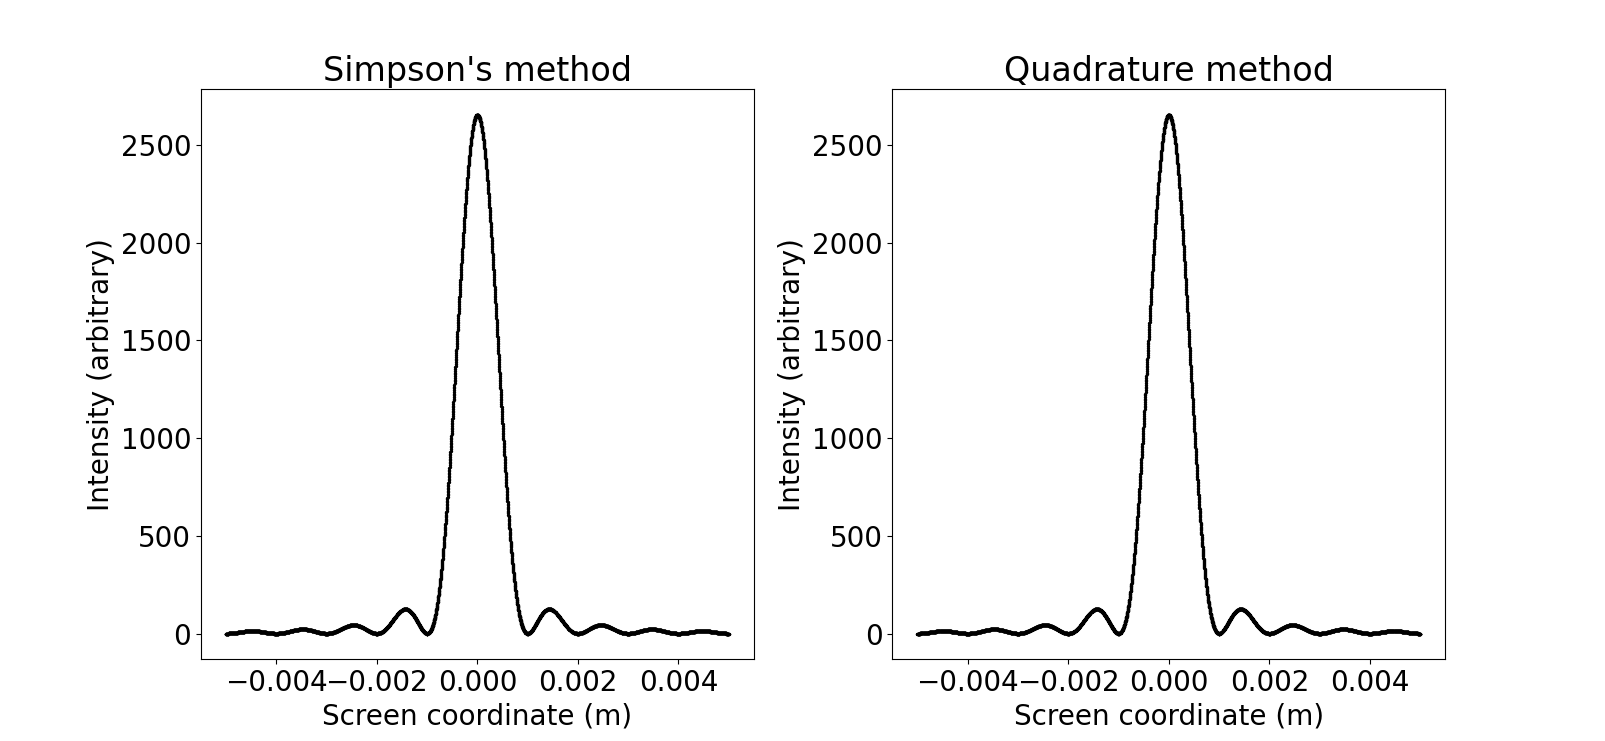
\includegraphics[width=1\linewidth]{./assets/diffraction_1d/simps_quad_ff.png}
	\caption{Far-field diffraction shown as light intensity as a function of screen coordinate. Left: Simpson's method for numerical integration. Right: quadrature method for numerical integration.}%
	\label{fig:simps_quad_ff.png}
\end{figure*}

For part (b), 500 points were generated for each plot of of
Fig.~\ref{fig:aperture_width_effects}, which shows that increasing the aperture
width increases the peak intensity of the central maximum and decreases the
width of the central maximum. Assuming the relationship is $I_0 \propto d_a^m$,
it is quadratic as $m$ is the slope of the logarithmic plot on the left, which
is 2.00 to 3 significant figures. This models the physical phenomenon wherein
the light intensity which comes through the aperture and diffracted onto the
screen is proportional to the square of the aperture width. Meanwhile, assuming
the relationship is $\sin{\theta} \approx \theta \propto d_a^n$ ($\theta$ being
the angular half-width), the width of the central maximum $2\theta$ is inversely
proportional to the aperture width, as the slope of the logarithmic plot on the
right is $n = -1.00$ to 3 significant figures. This models the physical
phenomenon where the angular half-width is given as $\theta \sim \lambda /
	d_a$.

\begin{figure*}[htpb] \centering
	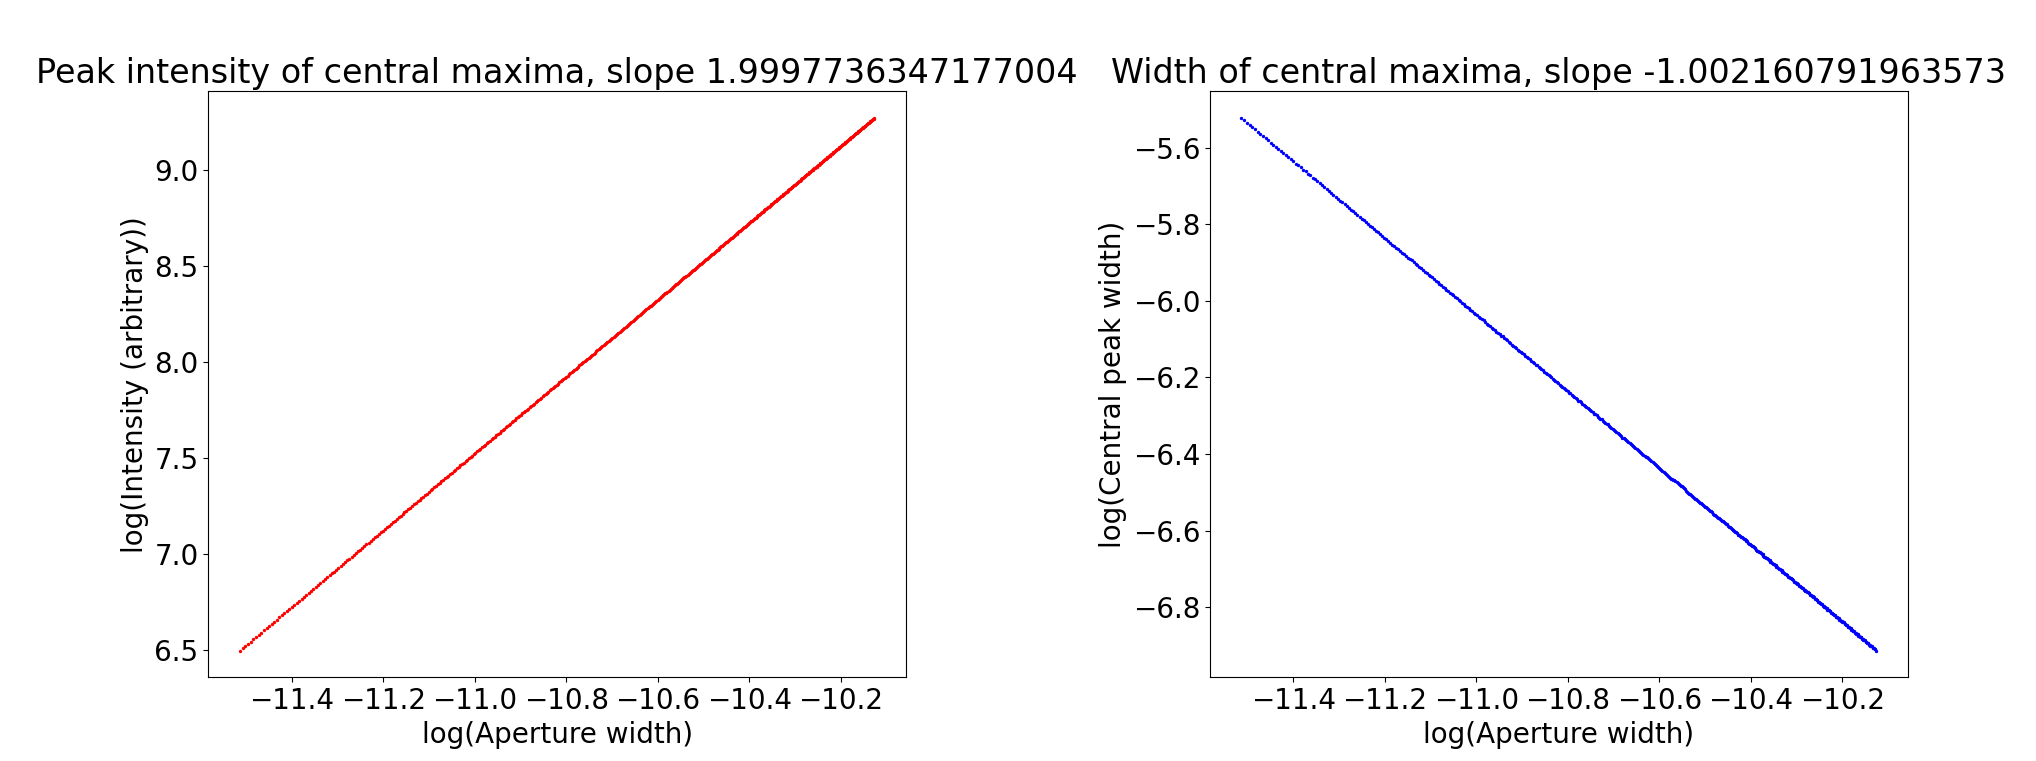
\includegraphics[width=1\linewidth]{./assets/diffraction_1d/aperture_width_effects_log.png}
	\caption{Left: log-log plot of central peak intensity as a function of aperture width. Right: log-log plot of central width as a function of aperture width.}%
	\label{fig:aperture_width_effects}
\end{figure*}

Similarly, 500 data points were generated for
Fig.~\ref{fig:screen_distance_effects}, which shows that increasing the screen
distance decreases the intensity of the central maximum and increases the width
of the central maximum. Assuming the relationship is $I_0 \propto z^o$, it
satisfies the inverse square law as $o$ is the slope of the plot on the left,
which is -2.00 to 3 significant figures. This models the physical phenomenon
where the intensity of light follows the inverse square law $I \propto 1/z^2$
where z is the distance between the light source and the screen. Meanwhile,
assuming the relationship is $\sin{\theta} \approx {\theta} \propto z^p$, the
width of the central maximum $2\theta$ is proportional to $z$ as $p$ is the
slope of the plot on the right, which is 1.00 to 3 significant figures. This
models the physical phenomena where from symmetry, one can deduce that $\theta
	\propto \lambda z / d_a$.

\begin{figure*}[htpb] \centering
	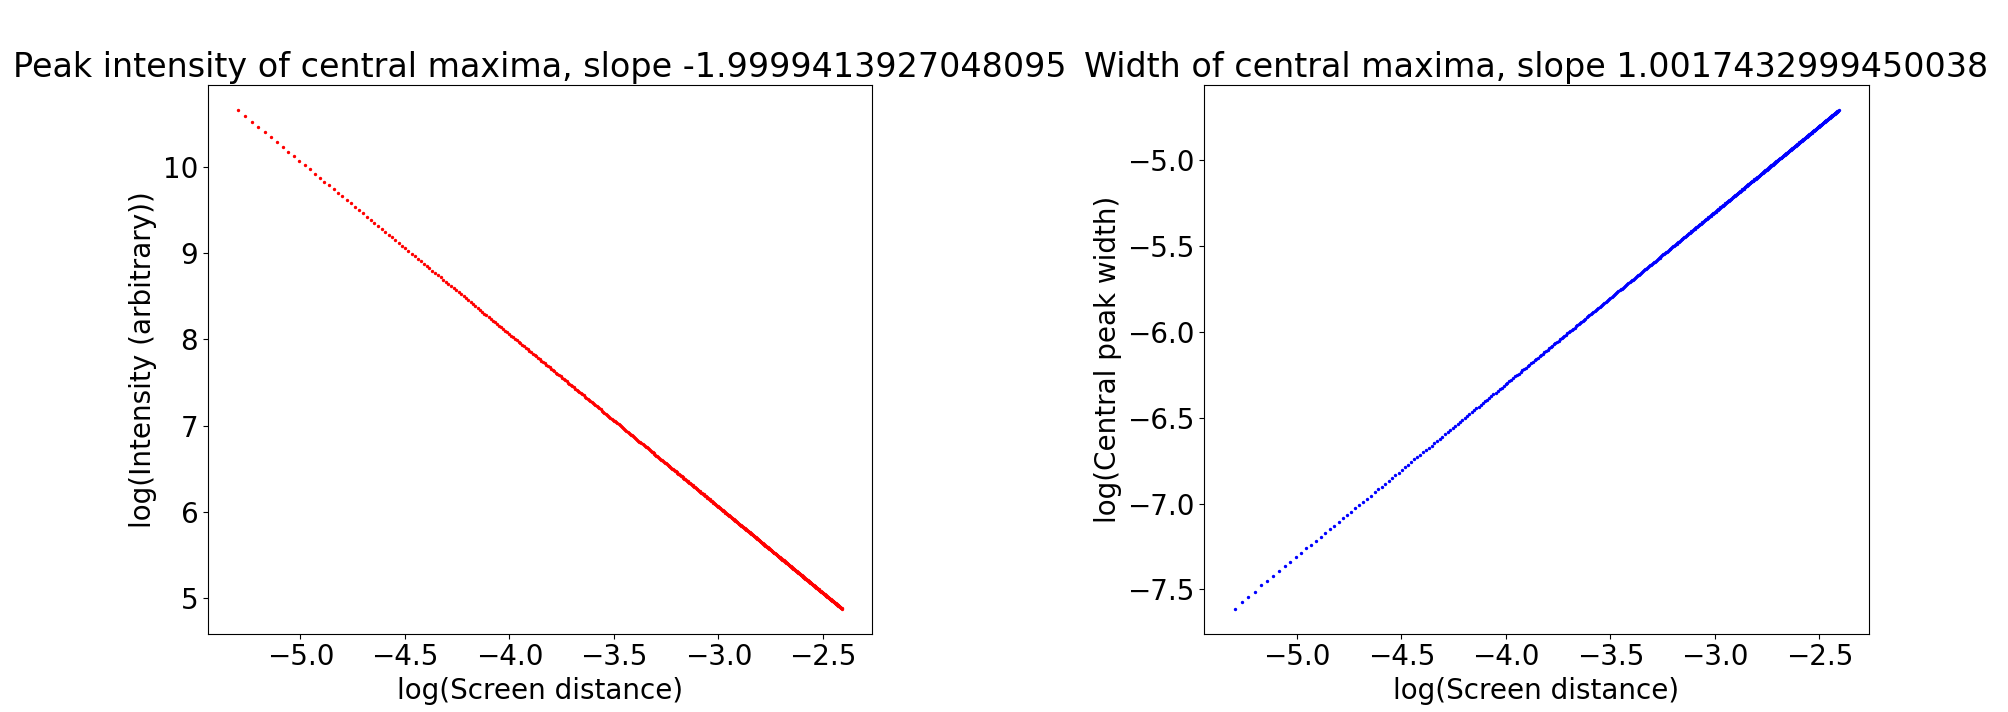
\includegraphics[width=1\linewidth]{./assets/diffraction_1d/screen_distance_effects_log.png}
	\caption{Left: log-log plot of central peak intensity as a function of screen distance. Right: log-log plot of central width as a function of screen distance.}%
	\label{fig:screen_distance_effects}
\end{figure*}

Next, far-field effects at different values of $N$ (data points for the
Simpson's method) were modelled (Fig.~\ref{fig:points_ff}). Only the pattern for $N > 101$ correctly
produces the pattern, as the next one at $N = 51$ (coloured purple), has a
second unexpected maxima far away from the screen centre. These unaccounted-for
maxima appear closer to the centre and more frequently as $N$ decreases. The
pattern does not `improve' for $N > 101$, showing that there is a lower
threshold for $N$ in which the Simpson's method is able to produce an accurate
integration.

\begin{figure*}[htpb]
	\centering
	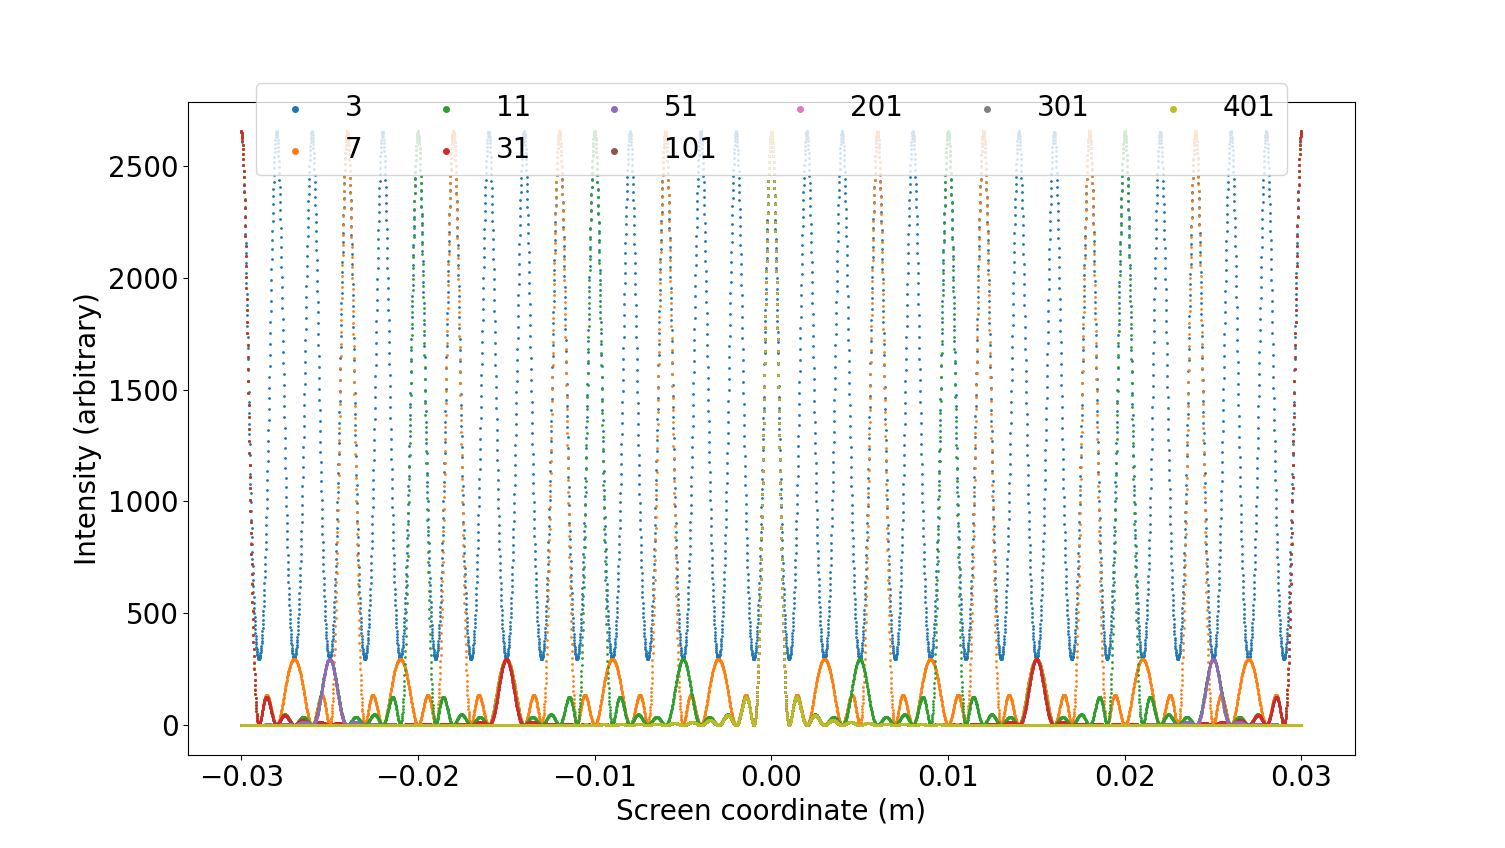
\includegraphics[width=1\linewidth]{./assets/diffraction_1d/points_ff.png}
	\caption{One dimensional far-field diffraction patterns at various sample sizes used in Simpson's numerical integration method, shown as light intensity as a function of screen coordinate.}%
	\label{fig:points_ff}
\end{figure*}

Next, near-field effects were observed by decreasing the screen distance $z$ to
\qty{3e-3}{\metre} while increasing the aperture width $d_a$ to
\qty{2e-3}{\metre}, and decreasing the area of the screen to integrate over
from \qty{-2e-2}{\metre} to \qty{2e-2}{\metre}. The sample size $N$ was also
increased to 401 for Fig.~\ref{fig:intensity_nf}. Whereas before, there was
only one central maximum, the pattern now resembles sets of adjacent maxima of
equal intensity at high intensities (the less-dense, tall peaks) to low
intensities (flatter, highly-dense peaks). Observed would be dark and bright
bands, whereas in the far-field approximation there would only be one central
band.

\begin{figure*}[htpb]
	\centering
	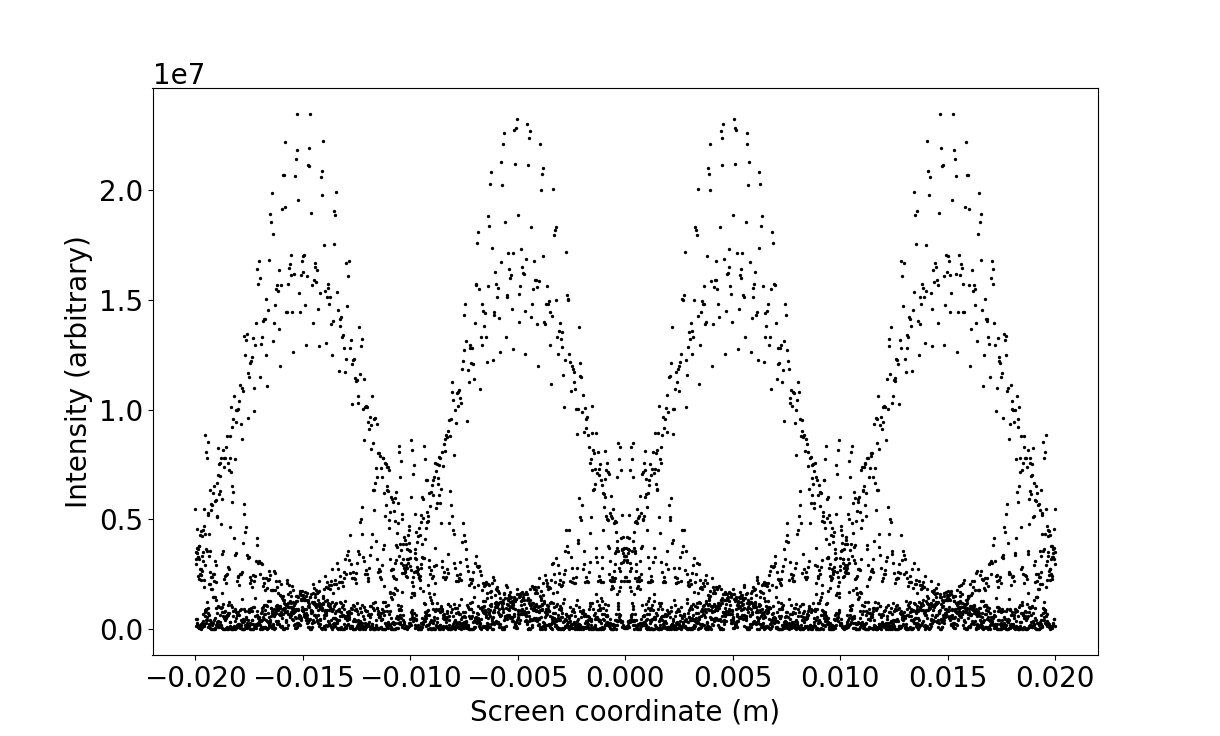
\includegraphics[width=1\linewidth]{./assets/diffraction_1d/intensity_nf_2.png}
	\caption{One dimensional near-field diffraction shown as light intensity as a function of screen coordinate.}%
	\label{fig:intensity_nf}
\end{figure*}

In the far-field approximation, $N = 101$ seemed to be the lower-bound to
produce an accurate diffraction pattern. In the near-field approximation, the
moss-coloured pattern ($N=401$) seen in Fig.~\ref{fig:points_nf} (the same in
Fig.~\ref{fig:intensity_nf}) differs from the grey-coloured pattern ($N=301$),
and successively lower $N$-patterns differ from the previous one. This shows
that near-field diffraction produces a more challenging integration which
requires more samples to accurately approximate. As most of the colour-coding
of each $N$ value can be seen on their own with few overlaps, the accuracy of
the Simpson's method for lower $N$ reduces significantly for near-field
approximation.

\begin{figure*}[htpb] \centering
	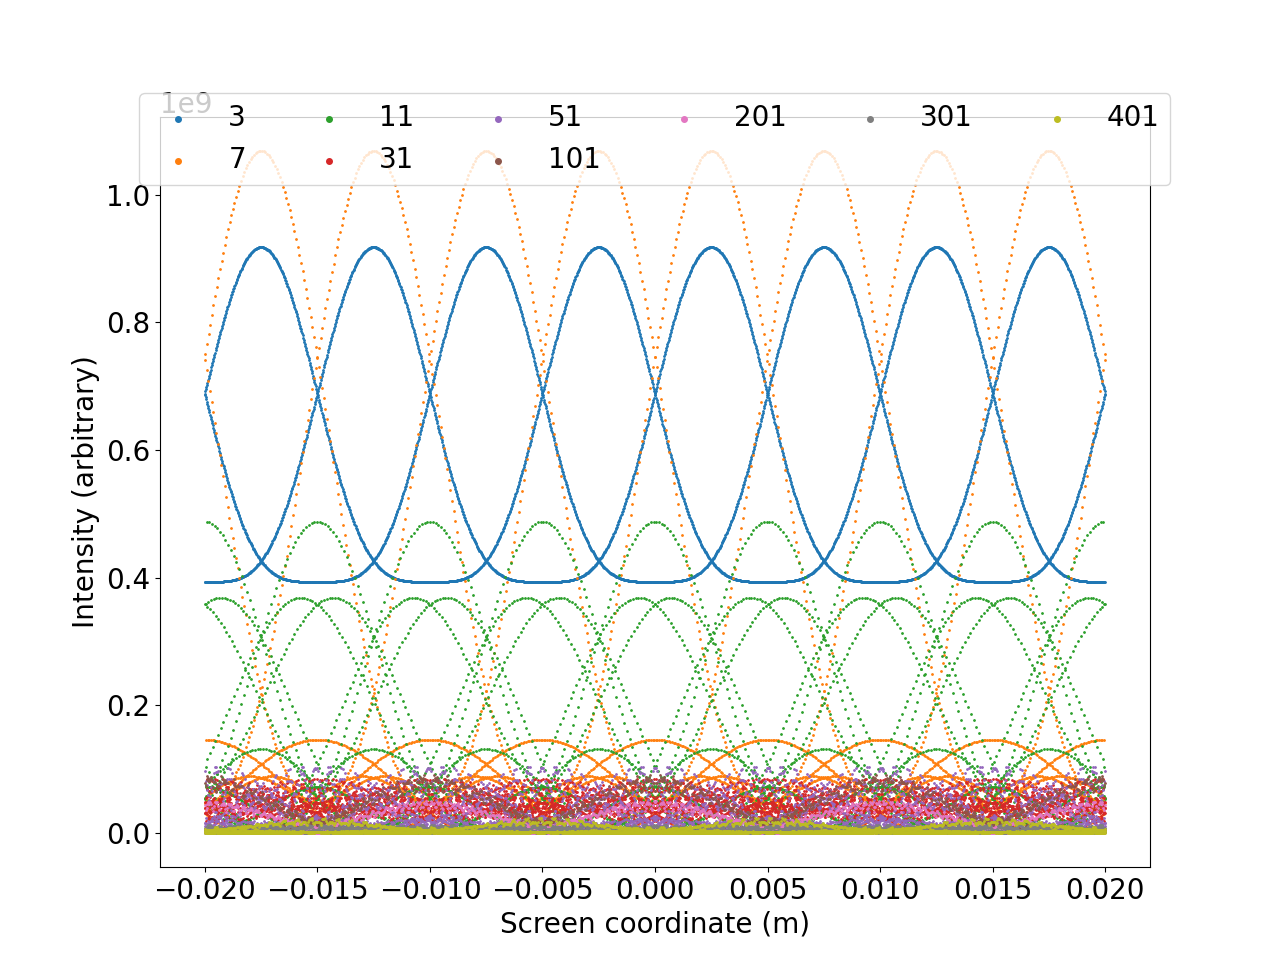
\includegraphics[width=1\linewidth]{./assets/diffraction_1d/points_nf.png}
	\caption{One dimensional near-field diffraction patterns at various sample sizes used in Simpson's numerical integration method, shown as light intensity as a function of screen coordinate.}%
	\label{fig:points_nf}
\end{figure*}

For part (c), square and rectangular apertures were modelled for near and
far-field effects (Fig.~\ref{fig:square_ap} and Fig.~\ref{fig:rect_ap}). This
requires integrating Eq.~\ref{eq:fresnel} in two dimensions. To get the
simulations to run for near-field, the screen size had to be reduced in order
for the code to run in reasonable timescale. Additionally, there were also
artefacts produced, as seen in Fig.~\ref{fig:rect_ap} (top left and top right),
which is potentially a loss of accuracy in
\lstinline{scipy.integrate.dblquad()} as the limits of integration (screen
size) were still too large in these two simulations. Regardless, near-field
effects were observed for screen distance $z$ at \qty{1e-4}{\metre} and below,
as arrays of bright and dark rectangular and squares can be observed. As
expected, for $z$ higher than this, the diffraction pattern becomes blurred and
a `central' bright `circle' or `oval' is seen instead as there is a loss in
resolution at this distance. Fainter peaks can be seen in both approximations,
similar to the 1-dimensional scenarios.

\begin{figure*}[htpb] \centering
	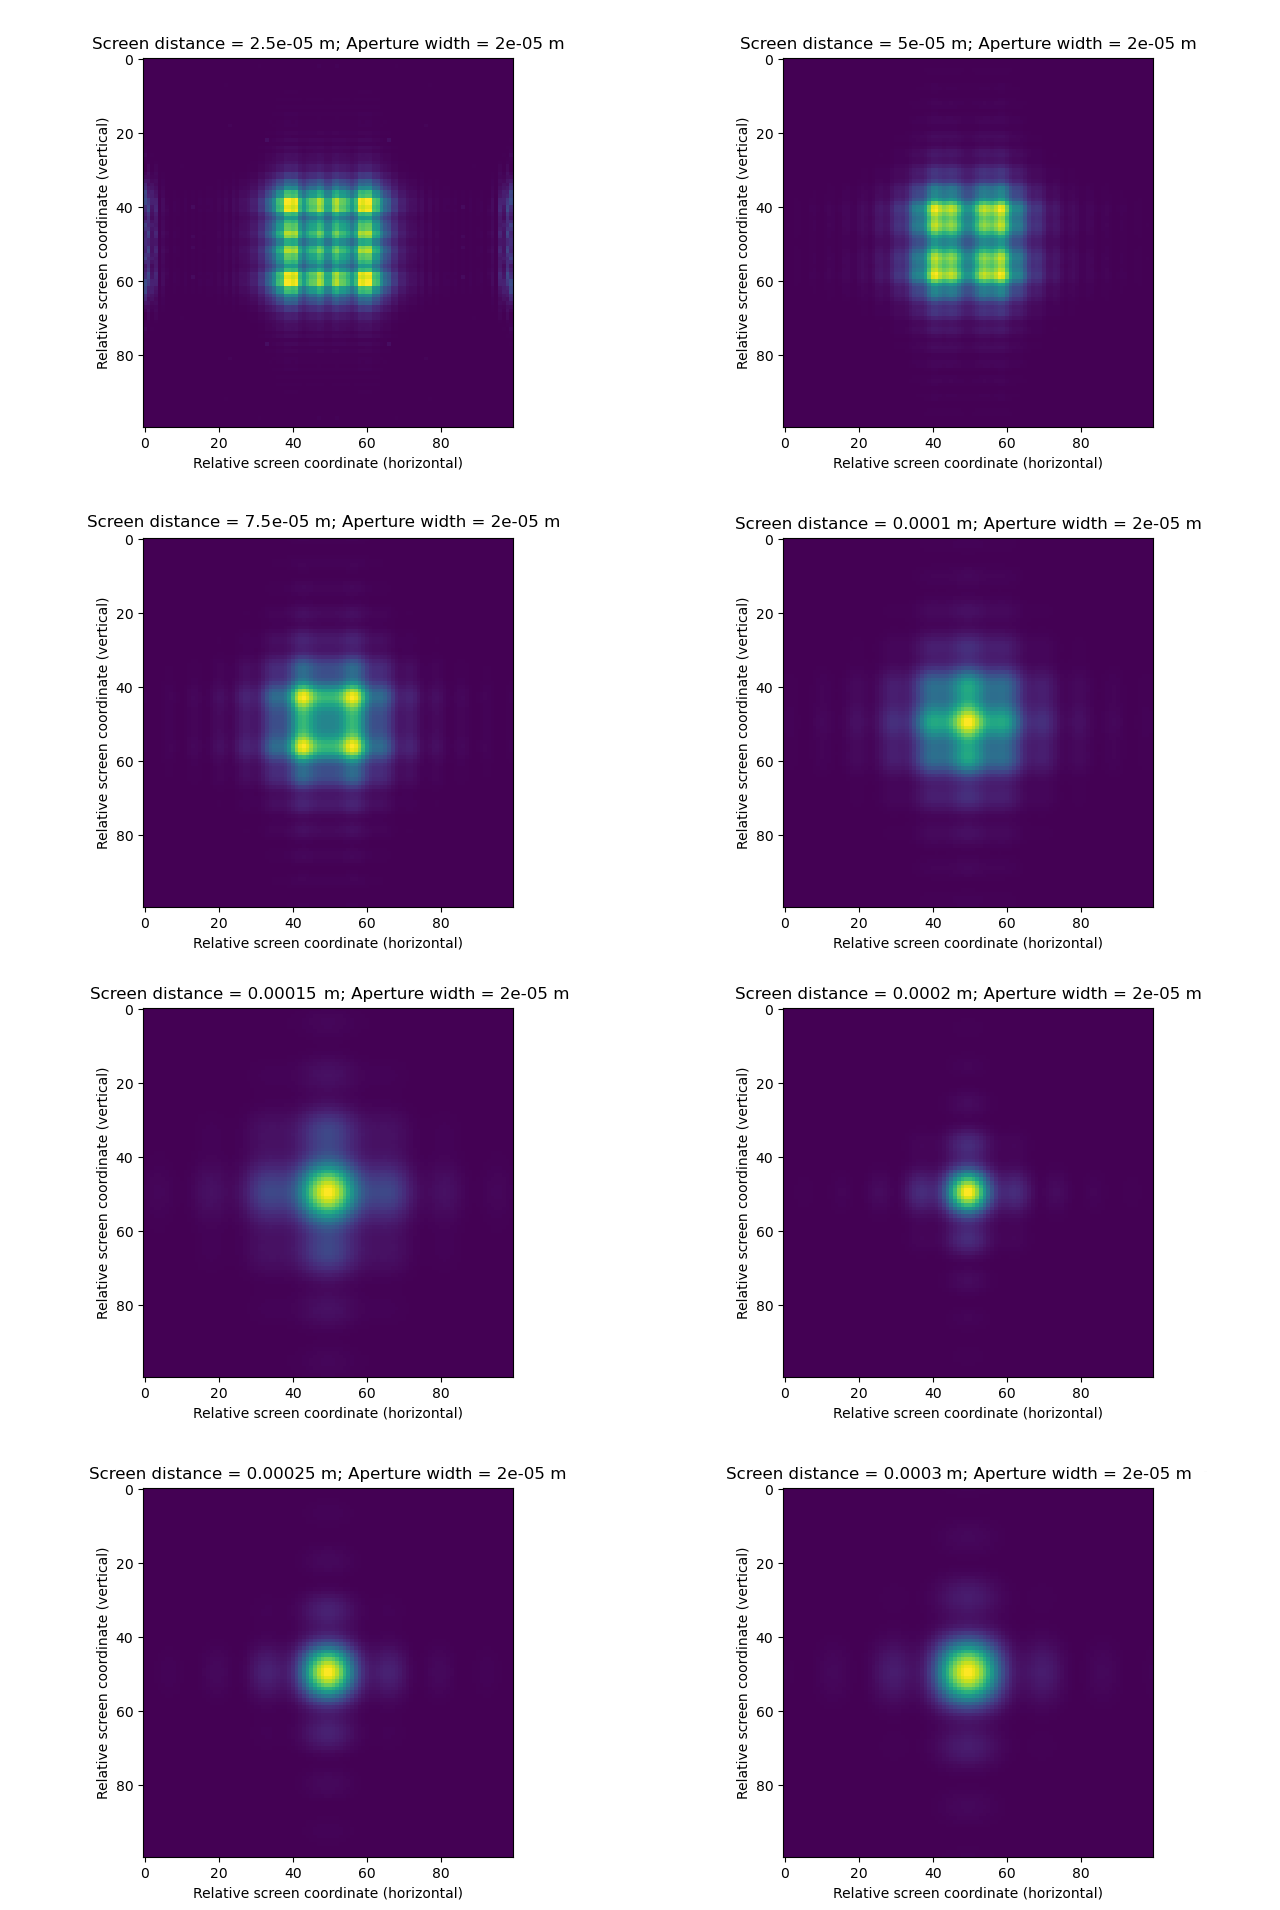
\includegraphics[width=1\linewidth]{./assets/square_apertures/combined.png}
	\caption{Two-dimensional diffraction through a square aperture for various screen distances.}%
	\label{fig:square_ap}
\end{figure*}

For part (d), limits were modified on the inner integral to change the aperture
into a circle, and the results (Fig.~\ref{fig:circ_ap}) display near-field
diffractions for $z$ below \qty{7.5e-5}{\metre}. An interesting phenomenon is
observed---there can be a dark or low intensity spot at the centre, instead of
a central maximum. This means that there is some phase destruction occurring
here. In the far-field approximation, there is always a central maximum. This
behaviour is characterised by the Fresnel number, $F$, where $F =
	R^2/z\lambda$. For even $F$ (integer), a central minimum is observed, for odd
$F$ (integer), a central maximum is observed, $F$ (non-integer) will be
in-between minimum and maximum intensity~\cite{fd}. For the top left aperture, $F =
	13.\dot{3}$, so in-between bright and dark, and for the top right aperture, $F
	= 8$, predicting a complete minimum, which is observed. Some artefacts were
also produced in the top left simulation, indicating some fine-tuning needed to
be done with the parameters being passed into
\lstinline{scipy.integrate.dblquad()}.

\begin{figure*}[htpb] \centering
	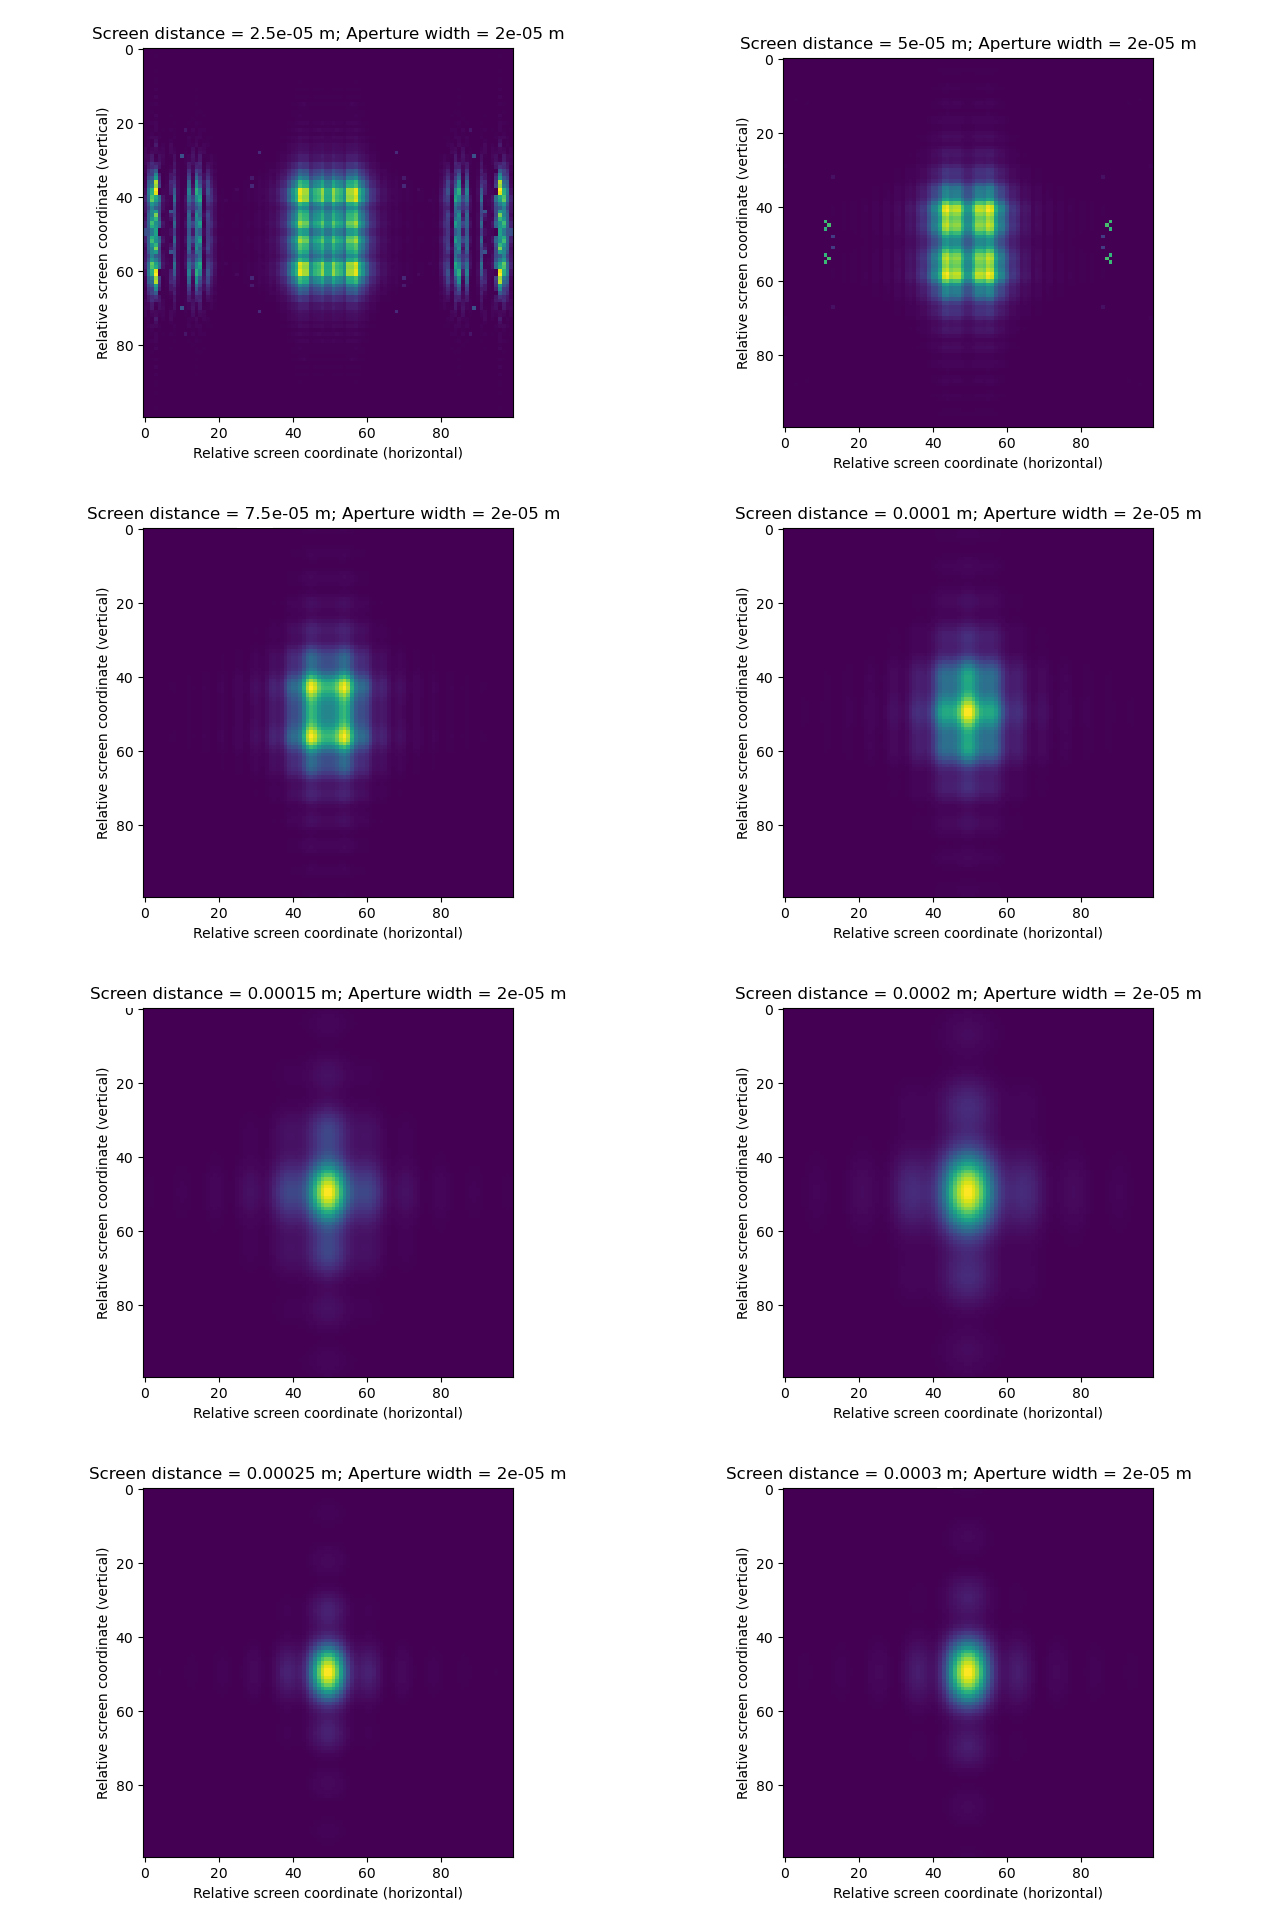
\includegraphics[width=1\linewidth]{./assets/rectangular_apertures/combined.png}
	\caption{Two-dimensional diffraction through a rectangular aperture for various screen distances.}%
	\label{fig:rect_ap}
\end{figure*}

\begin{figure*}[htpb] \centering
	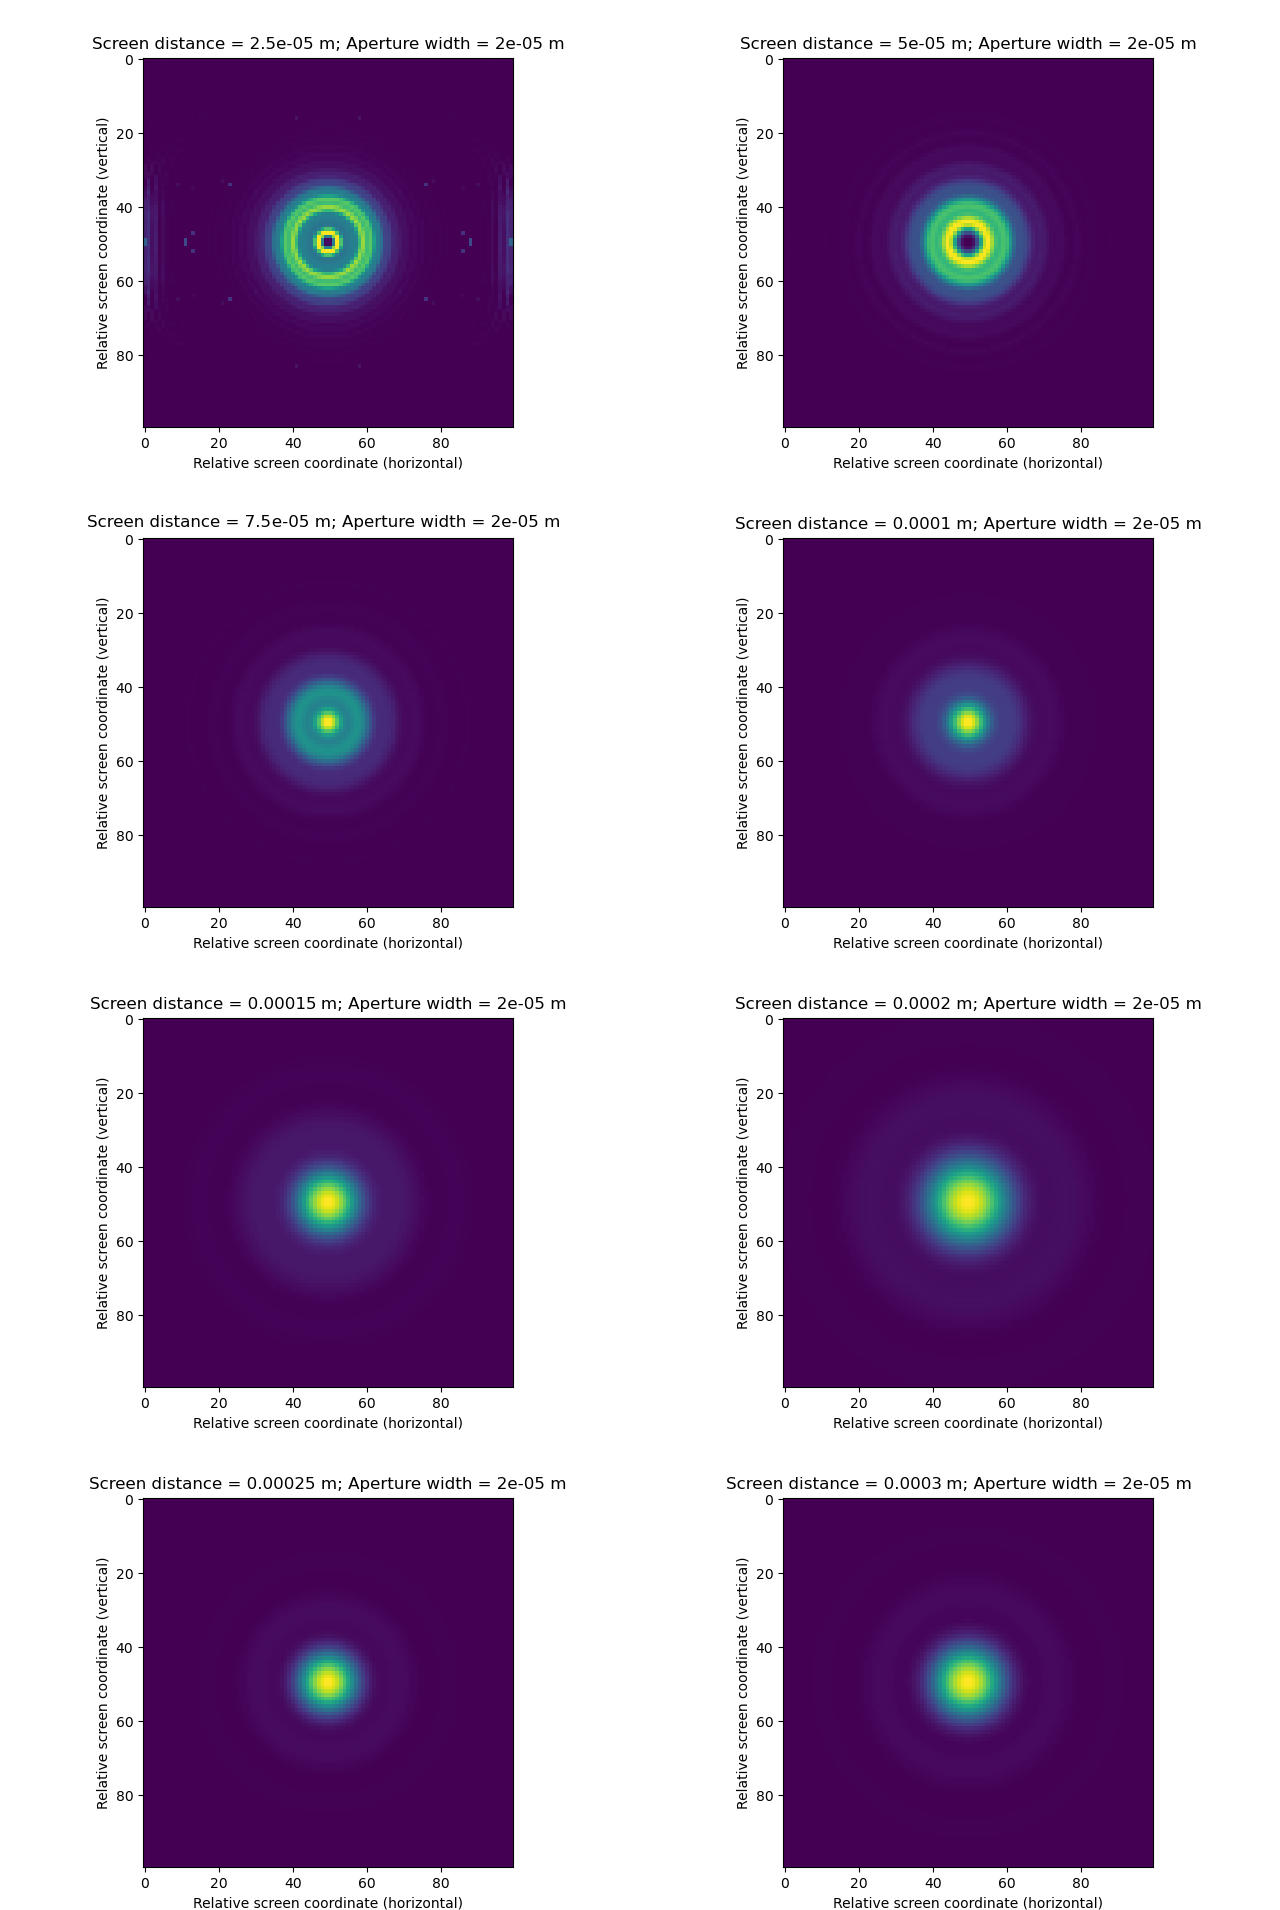
\includegraphics[width=1\linewidth]{./assets/circular_apertures/combined.png}
	\caption{Two-dimensional diffraction through a circular aperture for various screen distances.}%
	\label{fig:circ_ap}
\end{figure*}

\subsection{Conclusion}%
\label{sub:conclusion_1}

\noindent One-dimensional and two-dimensional diffraction patterns were
generated, both in the near-field regime and the far-field regime. The
distinction between these two regimes were decided qualitatively (visually).
Several physical phenomena were modelled with results as expected, namely the
relationships of $d_a$ and $z$ with $I_0$ (central intensity) and $2\theta$
(central width). Additionally, for the Simpson's integration method, a lower
sample size was needed to accurately model far-field diffraction compared to
near-field diffraction.

\section{PROBLEM 2: MONTE CARLO INTEGRATION}%
\label{sec:problem_2_wave_equation}

\subsection{Introduction}%
\label{sub:introduction_2}

\noindent Problem 2 involved solving integrals using the Monte Carlo method.
The situation is to find the ``volume'' of an n-dimensional sphere, for 2 to 10
dimensions.

Part (e) asked to evaluate a 2-dimensional integral using the Monte Carlo
approach to find the area of a unit circle. Part (f) asked to investigate the
error of the Monte Carlo method as a function of the sample size $N$ for the
previous calculation. Part (g) asked to extend the method onto higher
dimensions up to 10 to find the volumes of the unit-hyperspheres.

\subsection{Theory}%
\label{sub:theory_2}

\noindent The Monte Carlo method for solving integrals involves a sample of
random numbers to sample the shape or function of the region to be integrated.
The general equation is:

\begin{equation}
	\label{eq:monte_carlo_eq}%
	\int f\dd{V}\approx V\left(\langle f \rangle \pm\sqrt{\frac{\langle f^2 \rangle - \langle f \rangle ^2}{N}}\right)
\end{equation}

The volume of a hypersphere of $d$-dimension is analytically given by:

\begin{equation}
	\label{eq:hypersphere_vol}%
	V_d = \frac{2\pi r^2}{d}V_{d-2}
\end{equation}

\subsection{Method}%
\label{sub:method_2}

\noindent For part (e), the area of a unit circle can be found using the Monte
Carlo method. To constrain the samples to be within the circle, random numbers
were generated within a square, then the function $f$ in
Eq.~\ref{eq:monte_carlo_eq} simply return 0 if it lies outside the circle, or 1
if it lies inside.

For part (f), the convergence of the result is investigated. For a unit circle,
the area is $\pi$. The sample number $N$ was varied and its effects on the
error was calculated.

For part (g), similar methods from part (e) and (f) were used to calculate the
volume and the effect of $N$ on the errors for hyperspheres up to 10
dimensions.

\subsection{Results and discussions}%
\label{sub:results_and_discussions_2}

\noindent For part (e), the Monte Carlo method was performed with $N=500,000$. This
typically yields an area of 3.14 $\pm$ 0.00164 unit area to 3 significant
figures. Thus, it can obtain $\pi$ to 2 decimal places.

For part (f), Fig.~\ref{fig:mc_2} shows 9,999 points generated for $N$ from 50
to 500,000 (in increments of 50). On the left of the figure shows the
convergence of results as the sample size increases. As seen on the right of
the figure, the logarithm of the error decreases linearly with the logarithm of
$N$. Modelling the relationship between error and $N$ as $\textrm{Error}\propto
	N^p$, taking the logarithm of both error and $N$, and running a least squares
linear fit using \lstinline{numpy.polyfit} reveals the power $p$ as the slope.
In the 2D case, the slope was found to be -0.5, which means the error of the
Monte Carlo method varies with $1/\sqrt{N}$. This statistical model works as
expected and verifies Eq.~\ref{eq:monte_carlo_eq}.

\begin{figure*}[htpb] \centering
	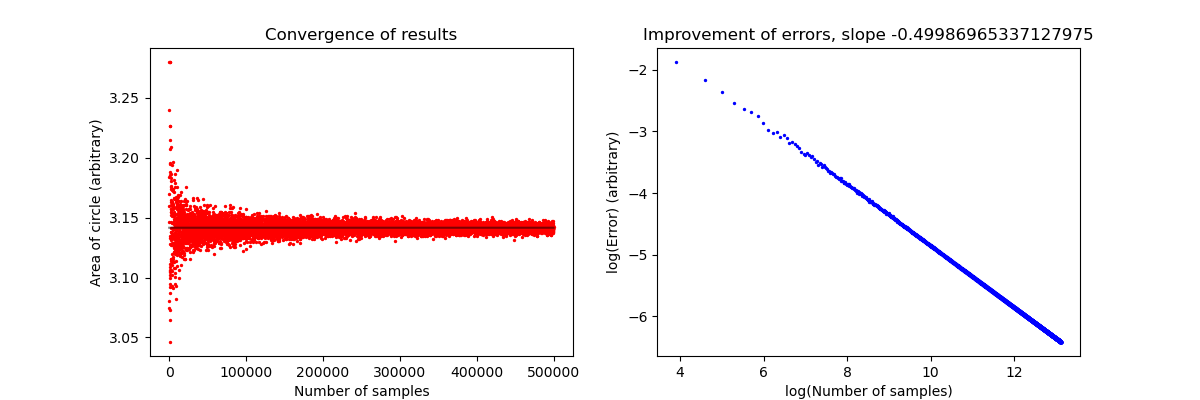
\includegraphics[width=1\linewidth]{./assets/monte_carlo/mc_2.png}
	\caption{Left: results of Monte Carlo integration as a function of sample size to estimate area of a two-dimensional circle. Right: log-log plot of errors of integration versus sample size.}%
	\label{fig:mc_2}
\end{figure*}

For part (g), the method was generalised up to 10 dimensions. The convergence
of results with $N$ is shown in Fig.~\ref{fig:mc_combined_results}, along with
the absolute errors in Fig.~\ref{fig:mc_combined_errors} (these plots are not
contained within the submitted code). Results converge towards the true value
as $N$ increases for all dimensions tested. The difference in rates of
convergence between each dimension is not clear from
Fig.~\ref{fig:mc_combined_results}. The reason is because for some
calculations, the volume ended up far from the true value, while for another
dimension this might not have happened. This made each plot scale differently,
so looking at all plots holistically, there is no pattern.

\begin{figure*}[htpb] \centering
	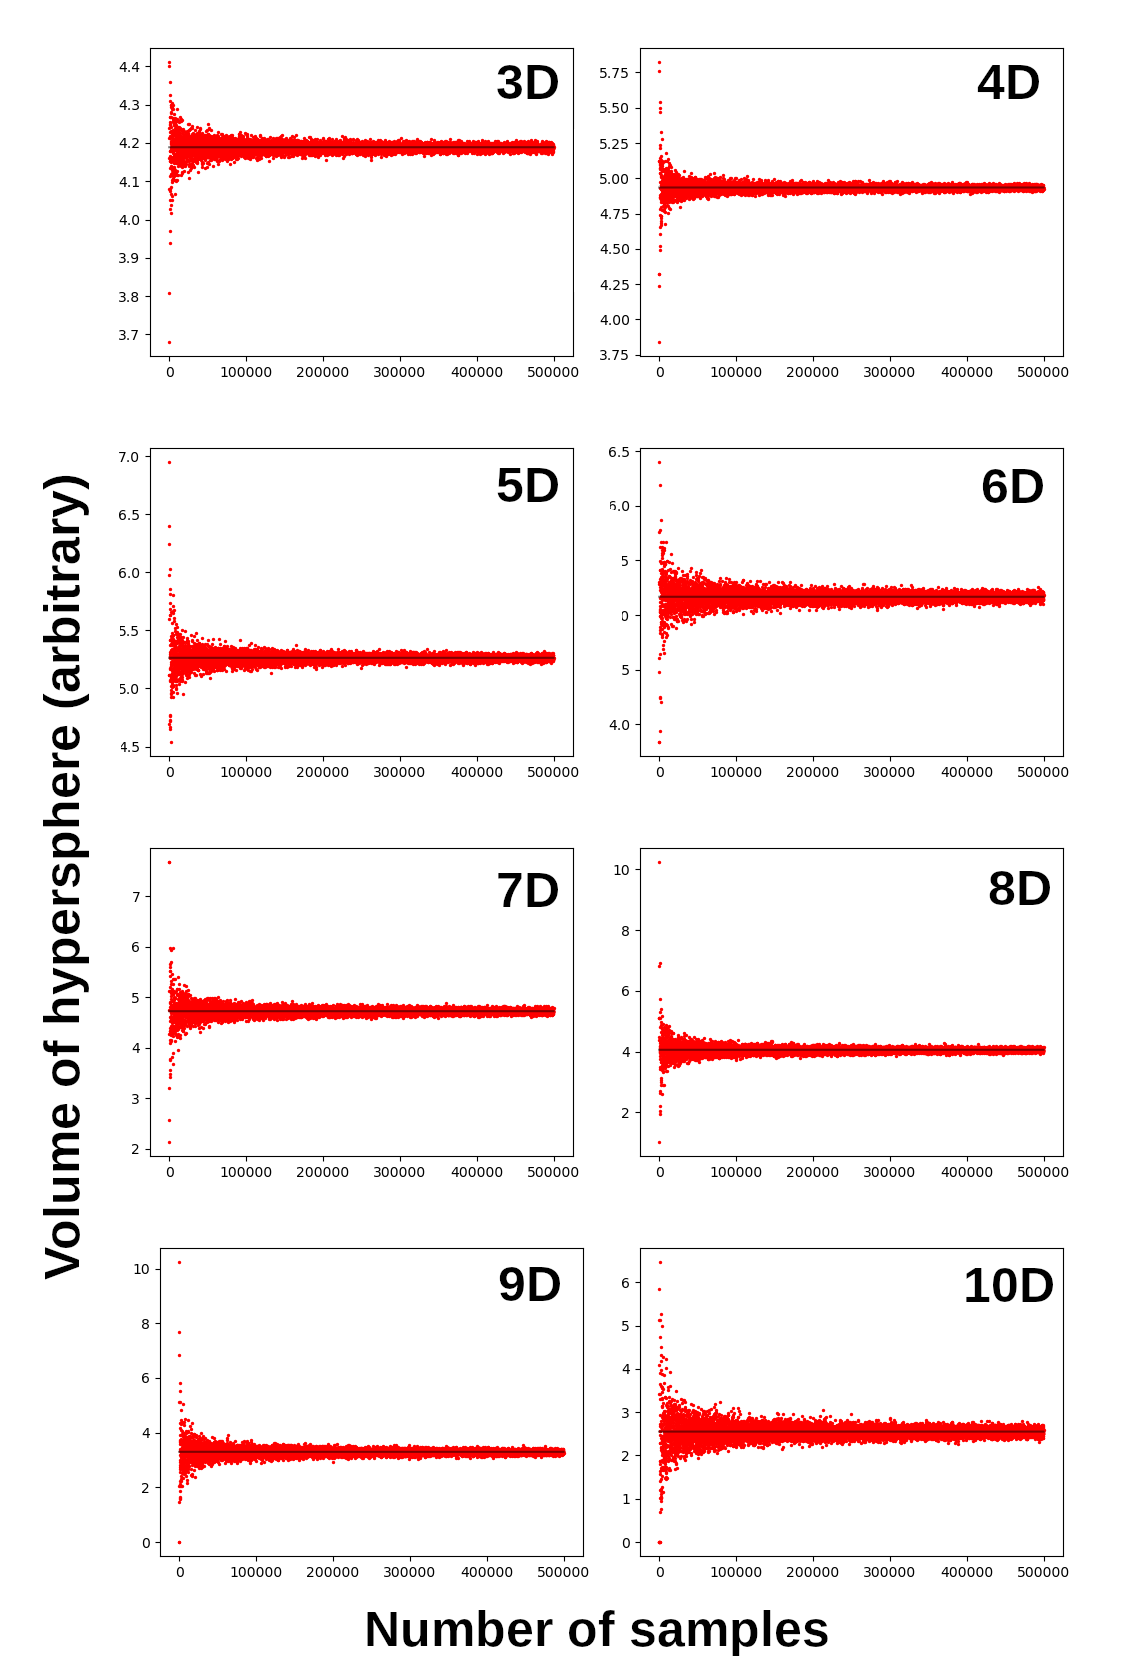
\includegraphics[width=1\linewidth]{./assets/monte_carlo/combined_results.png}
	\caption{The results of Monte Carlo integration as a function of sample size for number of dimensions $d$ from 3 to 10. The grey horizontal lines indicate the true value of convergence.}%
	\label{fig:mc_combined_results}
\end{figure*}

\begin{figure*}[htpb] \centering
	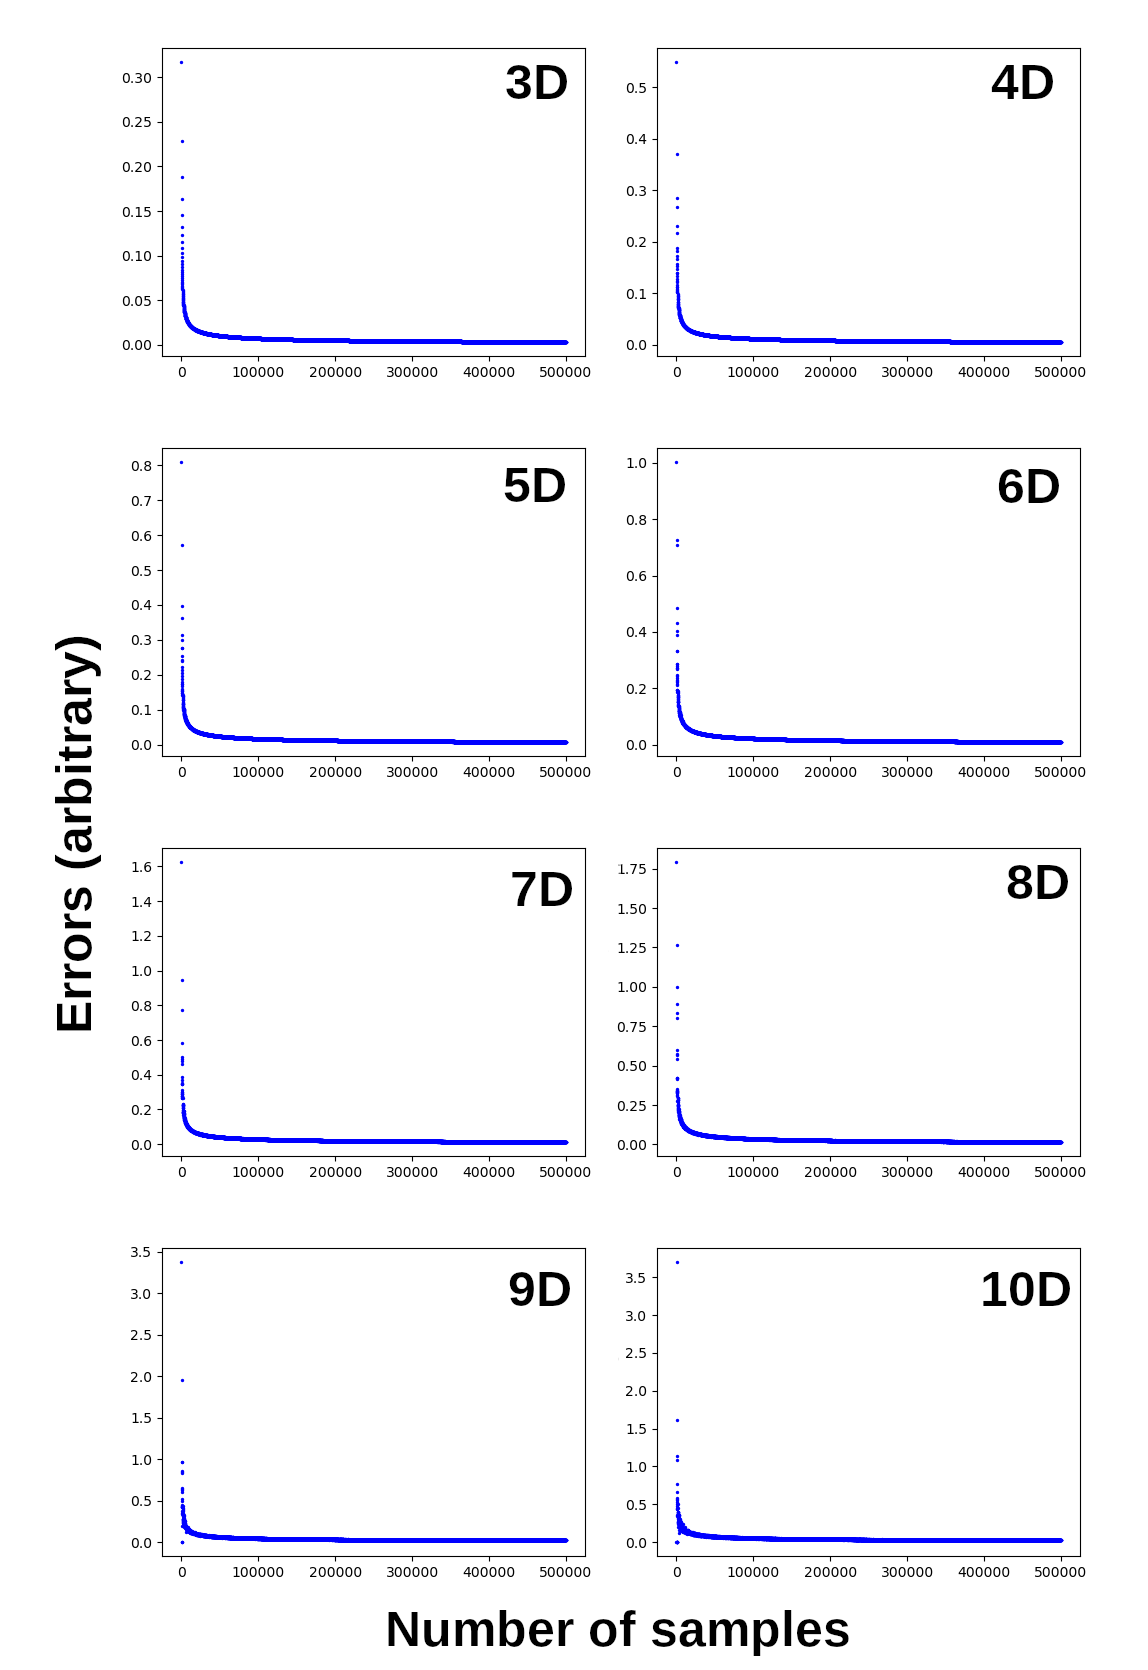
\includegraphics[width=1\linewidth]{./assets/monte_carlo/combined_errors.png}
	\caption{The absolute of errors of Monte Carlo integration as a function of sample size for number of dimensions $d$ from 3 to 10.}%
	\label{fig:mc_combined_errors}
\end{figure*}

Similar to the method in 2 dimensions, logarithmic error was plotted against
logarithmic $N$, as seen in Fig.~\ref{fig:mc_combined_log_errors}. For each
dimension, the slope of the logarithmic plot is approximated to be -0.5 to 1
significant figure, the table of all values is given in Table~\ref{tab:slope}.
This indicates the errors vary with $1/\sqrt{N}$ in all dimensions up to 10.
Looking at these plots holistically, it can be observed that the errors for
higher dimensions appear to correlate worse as the number of dimensions
increase, since the left `tail' of the plot streamlines into a straight line
slower.

\begin{table}
	\begin{tabular}{ c  c }
		Dimension $d$ & Power $p$ \\
		\hline
		1             & -0.500    \\
		2             & -0.500    \\
		3             & -0.500    \\
		4             & -0.500    \\
		5             & -0.500    \\
		6             & -0.500    \\
		7             & -0.499    \\
		8             & -0.500    \\
		9             & -0.499    \\
		10            & -0.497    \\
	\end{tabular}
	\caption{The gradient of log-log plots to estimate the relationship between the errors of Monte Carlo integration and sample size.}
	\label{tab:slope}
\end{table}

\begin{figure*}[htpb] \centering
	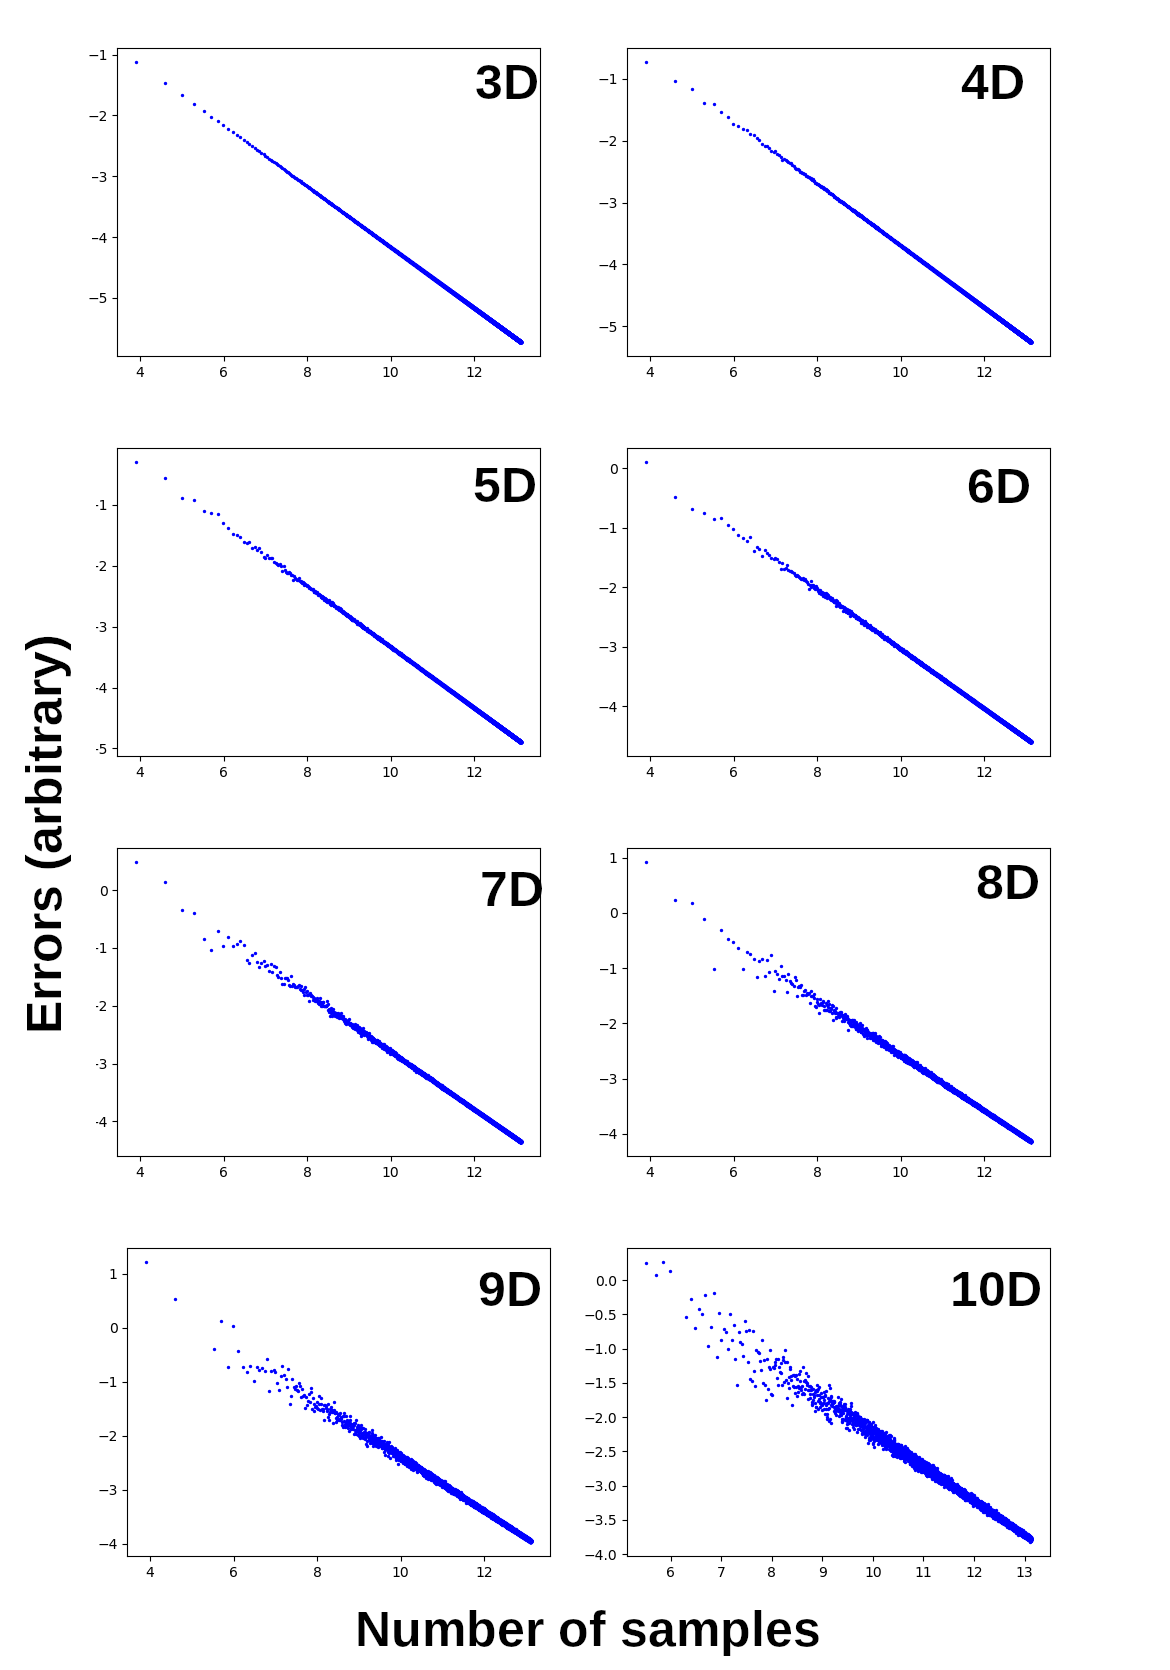
\includegraphics[width=1\linewidth]{./assets/monte_carlo/combined_log_errors.png}
	\caption{The log-log plot of errors of Monte Carlo integration versus sample size for number of dimensions $d$ from 3 to 10.}%
	\label{fig:mc_combined_log_errors}
\end{figure*}

One reason this could happen is the following: assuming the sample size $N$ is
now kept constant, as the number of dimensions $d$ increases, the volume of the
hypersphere decreases towards 0 very quickly (see Fig.~\ref{fig:nball_vol}),
while the volume of the hypercube which contains the hypersphere increases
($V_{\textrm{d}} = 2^d$ for a unit hypersphere). The result of this is the
fraction of $N$ that lies within the hypersphere
$n_{\textrm{inside}}/n_{\textrm{total}}$ decreases as the $d$ increases. While
for any population of random variable, at large $N$, the central limit theorem
shows that the population is distributed normally. At low $N$, the mean and
variance is more sensitive to specific values. At higher $d$, at low values of
$N$, there might not be enough data points within the hypersphere due to the
fraction $n_\textrm{inside}/n_\textrm{total}$ being small compared to values at
lower $d$, perturbing the sample standard deviation from the true population
standard deviation. This leads to more perturbation is observed in the error
(which is proportional to the standard deviation) at lower values of $\log{N}$
as $d$ increases.

\begin{figure*}[htpb] \centering
	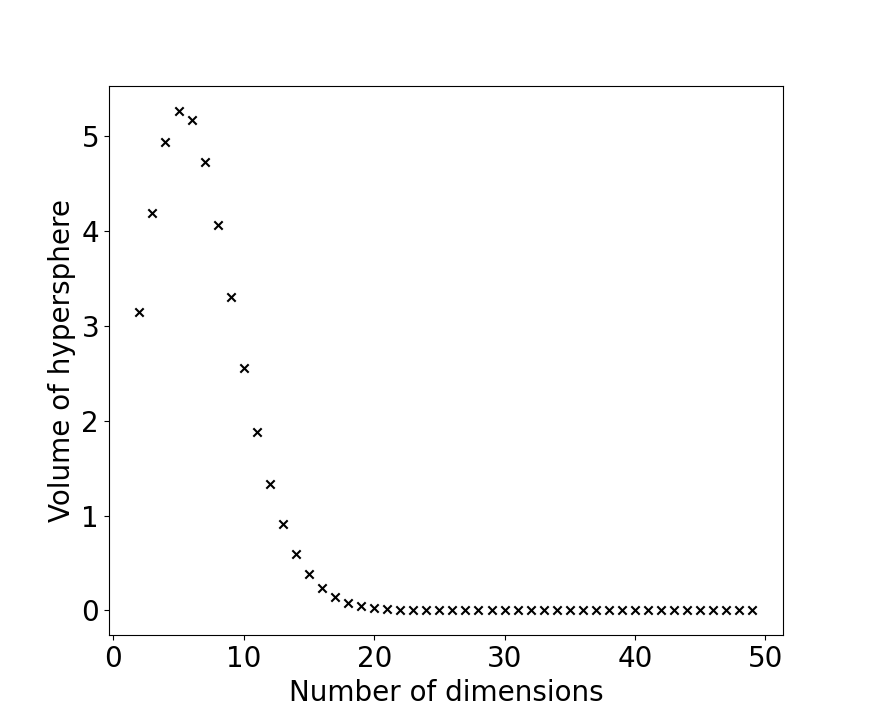
\includegraphics[width=1\linewidth]{./assets/monte_carlo/nball_vol.png}
	\caption{The volume of an $n$-ball or hypersphere as a function of the number of dimensions $d$. The peak value is at $d = 5$.}%
	\label{fig:nball_vol}
\end{figure*}

The Monte Carlo method utilised in part (e), (f), and (g) uses a pseudorandom
number generator (PRNGs). PRNGs are not \textit{truly random} as they are not
unpredictable. Instead, they only approximate a sequence of \textit{truly
	random} numbers, and remain deterministic by nature~\cite{ka}. There are many
methods to generate pseudorandom numbers, they tend to begin with an initial
value---a seed. This seed can be obtained truly randomly, however, the
algorithms that can be used to generate the numbers after the seed are
deterministic.

However, a disadvantage of PRNGs as a sampler in Monte Carlo integration is
that it might not cover the domain of interests thoroughly (all points might
not be equidistributed inside the hypercubes). Instead, quasirandom number
generators (Quasi-RNGs), which is less random than PRNGs, actually perform
better than PRNGs in terms of quicker convergence. This method is known as the
quasi-Monte Carlo method~\cite{qmc}. The Quasi-RNGs produce numbers with
\textit{low-discrepancy}~\cite{qrngs}. A sample of numbers are
\textit{equidistributed} if the discrepancy tends to 0 as the sample size $N$
goes to infinity~\cite{es}. An additional part (h) of this problem was added
which used the \lstinline{scipy.qmc.stats} library to generate a
low-discrepancy sample of points, and the convergence comparison between the
two is given by Fig.~\ref{fig:pseudo_quasi}. A total of 35,000 integrations
were performed, 5,000 at each $N$ value to find the area of a circle. It can be
seen that for both methods, the spread of values is on average centred around
the true value $\pi$, but the spread of the quasi-Monte Carlo method is in all
cases lower than the pseudorandom Monte Carlo method, indicating that
convergence happens quicker as the density of results near the actual value at
any given $N$ is higher for the quasi-Monte Carlo than the pseudorandom Monte
Carlo method.

\begin{figure*}[htpb] \centering
	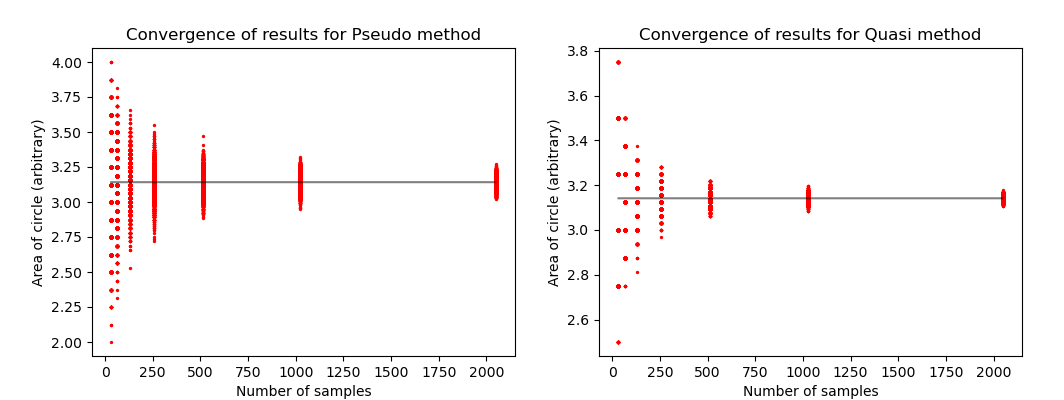
\includegraphics[width=1\linewidth]{./assets/monte_carlo/pseudo_quasi.png}
	\caption{Comparison between convergence Pseudo-Monte Carlo (left) and Quasi-Monte Carlo (right). Grey horizontal line indicates the actual value.}%
	\label{fig:pseudo_quasi}
\end{figure*}

\subsection{Conclusion}%
\label{sub:conclusion_2}

\noindent The Monte Carlo method was used to approximate the volumes of
hyperspheres for 2 to 10 dimensions. The method shows converge towards the
actual value for all dimensions, and the error of the method is shown to vary
with the inverse square root of the sample size. As one goes to higher
dimensions, the ratio of points within the hypersphere to points outside the
hypersphere decreases, meaning that at low values of $N$, the error (standard
deviation) is perturbed from the sample standard deviation. In general, this is
the pseudorandom Monte Carlo method, and it was qualitatively shown to converge
more slowly than the quasi-Monte Carlo method.

\begin{thebibliography}{2}

	\bibitem{fd} "Fresnel diffraction". Wikipedia. Retrieved 2023-02-12.
	\bibitem{ka} "Pseudorandom number generators". Khan Academy. Retrieved 2023-02-12.
	\bibitem{qmc} "Equidistributed sequence". Wikipedia. Retrieved 2023-02-12
	\bibitem{qrngs} "Low-discrepancy sequence". Wikipedia. Retrieved 2023-02-12.
	\bibitem{es} "Equidistributed sequence". Wikipedia. Retrieved 2023-02-12

\end{thebibliography}

\end{document}

% vim: fen fdm=syntax
